\documentclass[11pt]{article}
\usepackage{enumitem}
\usepackage{amsmath,amsthm,amssymb}
\usepackage{color}
\usepackage{graphicx}
\graphicspath{ {./images/} }

\begin{document}
\date{} 
\title{Prelab 4\\--\\\large CPE282 Fall 2020}
\author{Brennen Green}
\maketitle

\section*{Verilog Module}
\begin{center}
    \begin{verbatim}
    module prelab(input x, input y, input z, output f);
        always @(x or y or z)
            begin
            case({x,y,z})
                3'b000: f = 'b1;
                3'b001: f = 'b1;
                3'b010: f = 'b1;
                3'b111: f = 'b1;
                default: f = 'b0;
            endcase
            end
    endmodule
    \end{verbatim}
\end{center}

\section*{Schematics}
\begin{center}
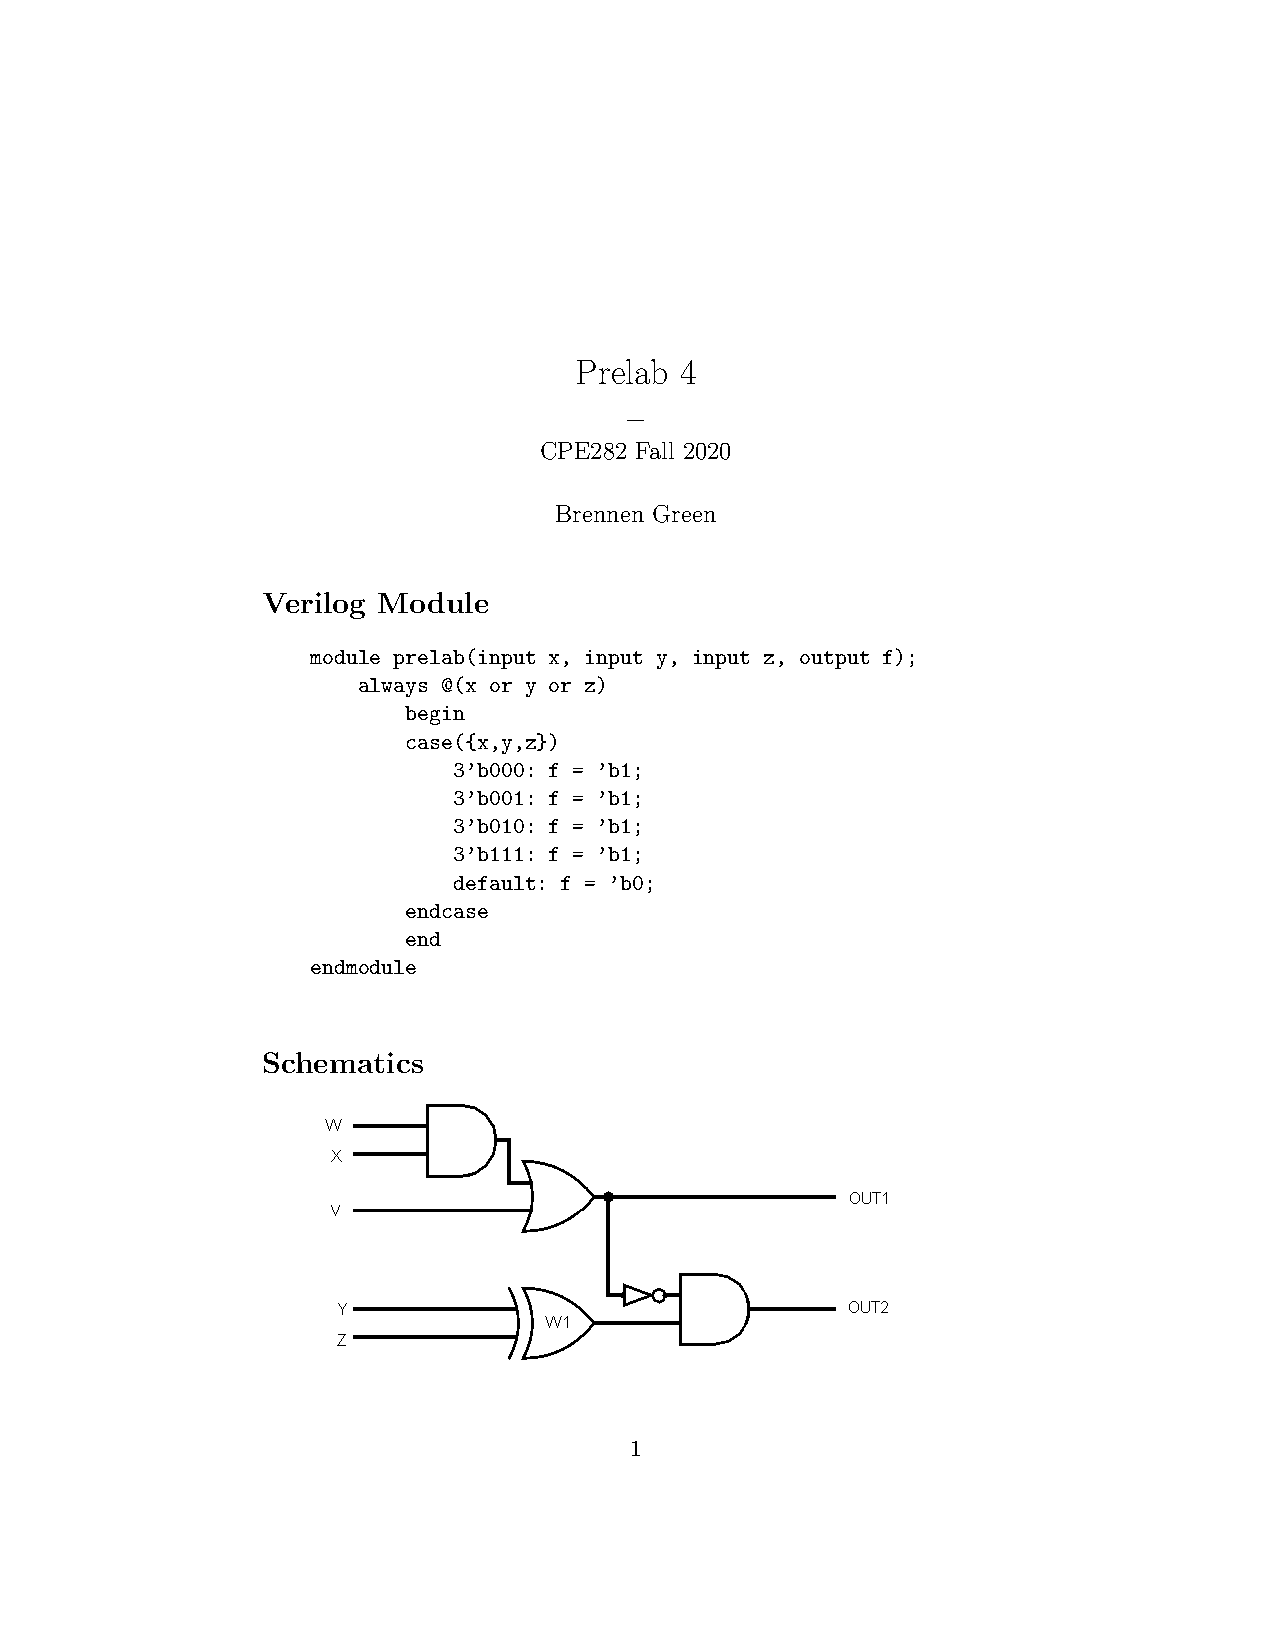
\includegraphics[width=10cm, keepaspectratio]{prelab}\newline
\end{center}


\end{document}

